\section{Optische Handgestenerkennung}
\label{sec:fallstudie}
\begin{figure}
    \centering
    \includegraphics[width=0.6\linewidth]{images/arduino_ex.png}
    \caption{Das Arduino-Board ATmega328P mit 3x3 Matrix von Lichtsensoren in Lego-Verpackung. Illustriert werden die möglichen Handgestentypen mit Ausnahme der Nullgeste.}
    \label{fig:arduino_ex}
\end{figure}
Diese Arbeit ist Teil einer Fallstudie zur Handgestenerkennung auf Low-End Mikrocontrollern von dem Institut für Telematik an der TUHH \cite{venzkeArticle}. Das Ziel ist die Handgestenerkennung in Echtzeit mit so wenig
Ressourcen wie möglich, damit die Produktion der einzelnen Module so kostengünstig wie möglich ist. Als Eingabe dient, je nach Modul, eine 3x3, bzw. 4x4, Matrix von Lichtsensoren. Abbildung \ref{fig:arduino_ex}
illustriert 4 Typen von Handgesten, die über den Mikrocontroller ausgeführt werden: Links nach Rechts, Rechts nach Links, Oben nach Unten, Unten nach Oben. Zudem wird zwischen Handgesten und Nullgsten, d. h.
invalide Handgesten. Die bisherigen Arbeiten haben sich mit künstlichen neuronalen Netzen beschäftigt. Dessen Prozessablauf zur Gestenerkennung lässt sich im Grunde auf 3 Schritte zusammenfassen.
\begin{enumerate}
    \item Extrahiere einen Gestenkandidaten.
    \item Vorverarbeite den Gestenkandidaten.
    \item Wende das Modell auf die vorverarbeiteten Gestenkandidaten an.
\end{enumerate}

\section{Exrahieren von Gestenkandidaten}
\label{sec:gesture_extraction}
Die Lichtsensorenmatrix liefert einen kontinuierlichen Strom an Bildern. Als Gestenkandidat wird eine Folge von Bildern definiert, die
ein Ereignis einschließt. In diesem Fall wird das Ereignis durch die Veränderung im gleitenden Mittelwert der Helligkeit definiert. Sobald der gleitende Mittelwert unterschritten wird, wird ein Gestenkandidat
angefangen aufgenommen zu werden. Sobald die Lichtverhältnisse zu dem Wert zurückkehren, wird die Aufnahme beendet. Der gleitende Mittelwert wird immer angepasst, wenn kein Gestenkandidat aufgenommen wird, um
sich den verändernden Lichtverhältnissen anzupassen. Da leichte Veränderungen natürlich sind, muss eine Toleranzgrenze von 10\% unter- und überschritten werden, damit die Aufnahme gestartet, bzw. beendet wird.
Die Folge ist, dass der Anfang und das Ende nicht vollständig ist. Aus diesem Grund schlug Kubik zusätzlich vor am Anfang und Ende weitere Bilder anzufügen \cite{kubikThesis}.
\begin{figure}
    \usetikzlibrary{arrows,automata,positioning}
    \centering
    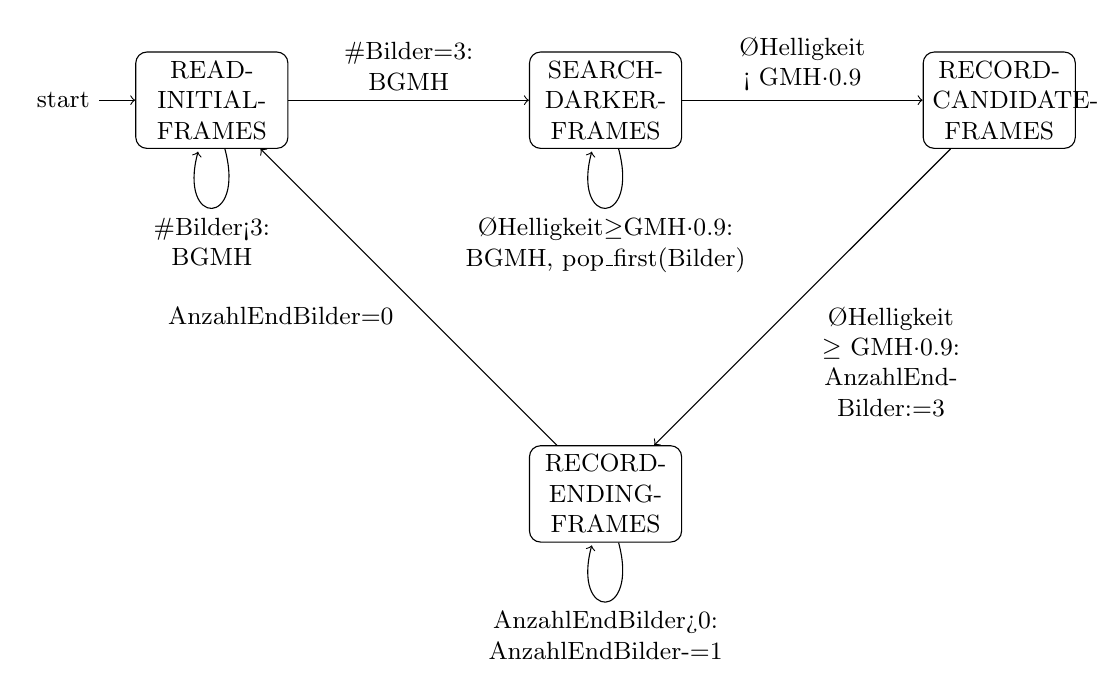
\begin{tikzpicture}[
        block/.style={
        draw,
        fill=white,
        text width=0.14*\columnwidth,
        anchor=west,
        minimum height=1cm,
        rounded corners
        },
        font=\small,
        on grid, auto,
        node distance=5cm
    ]
        \node [block,align=center,initial] (s0) {READ-INITIAL-FRAMES};
        \node [block,align=center] (s1) [right of=s0] {SEARCH-DARKER-FRAMES};
        \node [block,align=center] (s2) [right of=s1] {RECORD-CANDIDATE-FRAMES};
        \node [block,align=center] (s3) [below of=s1] {RECORD-ENDING-FRAMES};
        \path [->, text width=2cm, align=center] (s0) edge [loop below] node {\#Bilder<3: BGMH} (s0);
        \path [->, text width=2cm, align=center] (s0) edge node {\#Bilder=3: BGMH} (s1);
        \path [->, text width=4cm, align=center] (s1) edge [loop below] node {ØHelligkeit$\geq$GMH$\cdot 0.9$: BGMH, pop\_first(Bilder)} (s1);
        \path [->, text width=3cm, align=center] (s1) edge node {ØHelligkeit < GMH$\cdot 0.9$} (s2);
        \path [->, text width=2cm, align=center] (s2) edge node {ØHelligkeit $\geq$ GMH$\cdot 0.9$: AnzahlEndBilder:=3} (s3);
        \path [->, text width=3cm, align=center] (s3) edge [loop below] node {AnzahlEndBilder>0: AnzahlEndBilder-=1} (s3);
        \path [->, text width=3cm, align=center] (s3) edge node {AnzahlEndBilder=0} (s0);
    \end{tikzpicture}
    \caption{Die Implementierung von Dr. Marcus Venzke des Algorithmus von Kubik, um Gestenkandidaten zu erkennen. BGMH steht für die Aktion \glqq \textbf{B}erechnung \textbf{G}leitender \textbf{M}ittelwert der \textbf{H}elligkeit\grqq und GMH steht für die Variable \glqq \textbf{G}leitender \textbf{M}ittelwert der \textbf{H}elligkeit\grqq.}
    \label{fig:venzkeAlgoImpl}
\end{figure}
\newline
\newline
Abbildung \ref{fig:venzkeAlgoImpl} zeigt die konkrete Implementierung dieses Algorithmus mit einem Zustandsautomaten, der von Dr. Marcus Venzke entwickelt wurde. In jedem Zustand wird das aktuelle Bild dem Puffer angefügt.
Der Automat verbleibt im Zustand \texttt{READ-INITIAL-FRAMES} bis der Puffer drei Bilder enthält. Dabei wird stets der gleitende Mittelwert der Helligkeit angepasst. Anschließend geht der Automat in den Zustand
\texttt{SEARCH-DARKER-FRAMES} über, indem immer das erste Bild aus dem Puffer entfernt wird, da lediglich drei Bilder jeweils vor dem Aufnehmen und nach dem Aufnehmen des
Gestenkandidaten angefügt werden sollen. Außerdem wird weiterhin der gleitende Mittelwert angepasst. Sobald die Durchschnittshelligkeit 90\% des gleitenden Mittelwerts unterschreitet wird die Aufnahme begonnen.
Der Automat geht in den Zustand \texttt{RECORD-CANDIDATE-FRAMES} über. Dort verbleibt der Automat solange bis die Durchschnittshelligkeit 90\% des gleitenden Mittelwerts überschritten wird, woraufhin der Automat
in den Zustand \texttt{RECORD-ENDING-FRAMES} über geht. Dort werden die letzten drei Bilder dem Puffer angehängt. Sobald drei Bilder angehängt wurden, wird der Puffer dem Klassifizierer übergeben und anschließend
der Zustandsautomat zurückgesetzt. Daraufhin geht der Automat in den initialen Zustand wieder über.
\subsection{Skalieren des Gestenkandidaten}
\label{sec:scaling}
Ein Gestenkandidat besteht aus einer variablen Anzahl an Bildern. Durch die künstlich angefügten Bilder am Anfang und Ende sind es mindestens 8 Bilder. Kubik erkannte, dass ein neuronales Netz eine feste Anzahl an
Eingaben hat und diskutierte verschiedene Ansätze.
\newline
\newline
Er verwarf die Idee den Puffer mit irrelevanten Bildern oder Nullen auszufüllen, Bilder zu duplizieren oder Teile des Gestenkandidaten zu verwerfen, da dadurch
nicht die vollständige Geste auf die Eingangs-Ebene des NN abgebildet werden würde, oder dass die Geste womöglich verzerrt wäre.
\newline
\newline
Aus diesem Grund hat Kubik sich für lineare Interpolation auf eine fixe Anzahl von 20 Bildern entschieden, wenn weniger als 20 Bilder vorhanden sind. Wenn mehr als 20 Bilder vorhanden sind,
werden 20 Bilder gleichverteilt ausgewählt \cite{kubikThesis}. Dieser Ansatz wurde auch von Anton Giese aufgegriffen, der sich in diesem Zusammenhang ebenfalls mit künstlichen neuronalen Netzen
beschäftigt hatte \cite{gieseThesis}.
\section{Trainings- und Testmenge}
\label{sec:synthetischeDaten}
\label{sec:testdaten}
Die Modelle werden auf Basis von aufgenommenen Daten trainiert und getestet. Die Aufnahmen beinhalten die fünf Handgestentypen, die mit unterschiedlichen Lichtverhältnissen aufgenommen wurden. Die Lichtverhältnisse
sind durch verschiedene Lichtquellen und Ausführungsdistanzen der Handgeste zur Kamera entstanden. Die Handgesten wurden mit der flachen Hand oder mit dem Finger in verschiedenen Geschwindigkeiten ausgeführt.
Die Datenmenge umfasst insgesamt 4792 Handgesten.
\newline
\newline
Listing \ref{lst:sampleGesture} zeigt ein Beispiel einer gespeicherten Handgeste von Links nach Rechts. Abbildung \ref{fig:sample_gesture} illustriert die Handgeste als Graustufenbild.
Jedes Bild wird durch einen Komma separierten Vektor von Zahlen dargestellt. Die letzte Zahl ist die Beschriftung der Handgeste.
\begin{lstlisting}[label=lst:sampleGesture,caption={Beispiel einer gespeicherten Handgeste von Links nach Rechts.}]
    ...
    665,683,669,690,627,670,672,611,557,1
    662,679,657,676,564,592,633,467,415,1
    645,653,583,627,549,483,598,474,230,1
    576,444,269,488,251,209,352,184,187,1
    361,254,123,343,130,82,304,83,36,1
    131,69,41,120,34,39,72,25,30,1
    49,71,174,61,45,206,40,45,110,1
    111,242,473,113,195,467,122,210,343,1
    272,559,637,304,518,639,401,553,562,1
    566,646,654,592,580,654,634,618,602,1
    ...
\end{lstlisting}
Um die Datenmenge zu vergrößern, können synthetische Daten erzeugt werden. Dabei werden aus einer aufgenommenen Handgeste Variationen durch Rotation und Rauschen generiert. Außerdem können Helligkeiten,
Kontraste und Gamma verändert werden \cite{venzkeArticle}.
\newline
\newline
Als Testmenge wird ein Teil der Datenmenge bezeichnet, der nicht zum Trainieren verwendet wird. Kubik hat Testdaten unter verschiedenen Lichtverhältnissen und Entfernungen zur Kamera aufgenommen. Klisch hat
daraus eine Testmenge erstellt, die von Klisch und Giese zur Verifikation verwendet wurden \cite{klischThesis, gieseThesis}. Klisch definiert die Klassifizierungsgenauigkeit gemäß \ref{klisch_metric}. Die
Klassifizierungsgenauigkeit ist das Verhältnis zwischen der Anzahl an korrekt klassifizierten Handgesten und der Anzahl der Einträge in der Testmenge.
\begin{align}
    accuracy = \frac{\#true\ positives}{\#total\ gestures}
    \label{klisch_metric}
\end{align}
\begin{figure}[h!]
    \centering
    \includegraphics[width=\linewidth]{images/sample_gesture_total.jpg}
    \caption{Illustration der Handgeste von Links nach Rechts aus Listing \ref{lst:sampleGesture}.}
    \label{fig:sample_gesture}
\end{figure}
\subsection{Gestenerkennung mit künstliche neuronalen Netzen}
Insgesamt gingen dieser Arbeit 4 Arbeiten voraus, die sich mit künstlichen neuronalen Netzen im Zusammenhang dieser Fallstudie beschäftigt hatten.

\subsubsection{Engelhardt}
Engelhardt führte die in \ref{sec:fallstudie} definierten Handgesten mit der Hand, einem Finger und 2 Finger unter verschiedenen Helligkeiten aus, auf Basis dessen seine Modelle trainiert und validiert wurden. Er
argumentiert, dass rekurrente neuronale Netze (RNN), Feedforward neuronale Netze (FFNN) und Long-Short-Term Memory neuronale Netze (LSTMNN) am besten geeignet für temporale Probleme seien. Convolutional neuronale
Netze (CNN) verwarf Engelhardt aufgrund der geringen Auflösung der Gesten und da die Faltung extrem Rechenaufwendig sei. Desweiteren verwarf er LSTMNN, da diese zu viel Rechenleistung und Speicherplatz
benötigen. Als Eingabewerte zu seinen RNNs und FFNNs diente eine Sequenz von 20 Bilder die zu 180 Werten konkatiniert wurden und auf Werte zwischen 0 und 1 normalisiert wurden. Als bestes Model stellte sich eines
seiner FFNNs heraus, das auf seinen Testdaten bis zu 99\% Erkennungsgenauigkeit erzielte. Außerdem erwies es sich als robust gegenüber Rauschen und Helligkeitsveränderungen im Vergleich zum RNN. Die Ausführungszeit
des FFNN belief sich auf 11,54 ms mit einem Verbrauch von 11 kB Flash-Speicher und 573 bytes RAM \cite{engelhardtThesis}.

\subsubsection{Kubik}

\subsubsection{Klisch}

\subsubsection{Giese}
